\documentclass[23 pt,margin=0.9in,innermargin=-4.5in,blockverticalspace=-0.25in]{tikzposter}
\geometry{paperwidth=43in,paperheight=32.5in}
\usepackage[utf8]{inputenc}
\usepackage{amsmath}
\usepackage{amsfonts}
\usepackage{amsthm}
\usepackage{amssymb}
\usepackage{mathrsfs}
\usepackage{graphicx}
\usepackage{adjustbox}
\usepackage{enumitem}
\usepackage{wrapfig}
\usepackage{mwe} % for placeholder images
\usepackage{comment}
\usepackage[backend=biber,style=numeric]{biblatex}
\usepackage{SUtheme}

%tikz
\usepackage{tikz}
\usetikzlibrary{arrows.meta,decorations.markings}
\tikzset{
  ->-/.style={decoration={
    markings,
    mark=at position #1 with {\arrow{>}}},
    postaction={decorate}}
}
\usetikzlibrary{calc}


\addbibresource{refs.bib}

% set theme parameters
\tikzposterlatexaffectionproofoff
\usetheme{SUTheme}
\usecolorstyle{SUStyle}
\usetitlestyle{Filled}

\usepackage[scaled]{helvet}
\renewcommand\familydefault{\sfdefault} 
\usepackage[T1]{fontenc}

\linespread{0.9}

\title{Braid Groups, and their Representations}
\author{Zih-Yu Hsieh \quad \quad Mentor: Choomno Moos}
\institute{University of California Santa Barbara, College of Creative Studies}
\titlegraphic{
\includegraphics[width=0.06\textwidth]{logo.png}}

% begin document
\begin{document}
\maketitle
\centering
\begin{columns}
    \column{0.32}
    \block{Introduction}{}

    \block{Braid Groups \& Mapping Class Groups}{ 
        \textbf{Def:} Braid group of $n$ strands $B_n$ is generated by $n-1$ elements $\{\sigma_1,...,\sigma_{n-1}\}$, satisfying \emph{Braid Relations}:
        \begin{itemize}
            \item $\sigma_i \sigma_j = \sigma_j \sigma_i$, if $|i-j|\geq 2$
            \item $\sigma_i \sigma_{i+1}\sigma_i = \sigma_{i+1}\sigma_i \sigma_{i+1}$ 
        \end{itemize}
        
        \textbf{Def:} Let $D_n$ be an $n$-punctured disk. The \emph{Mapping Class Group} $\mathfrak{M}(D_n)$ collects classes of isotopic self-homeomorphisms on $D_n$ that fixes disk boundary $\partial D$.

        \textbf{Ex:} The $i^\textmd{th}$ \emph{Half Twist} $\tau_i \in \mathfrak{M}(D_n)$ swaps the $i^\textmd{th}$ and $(i+1)^\textmd{th}$ punctures, while fixing the remaining ones.

        \begin{center}
            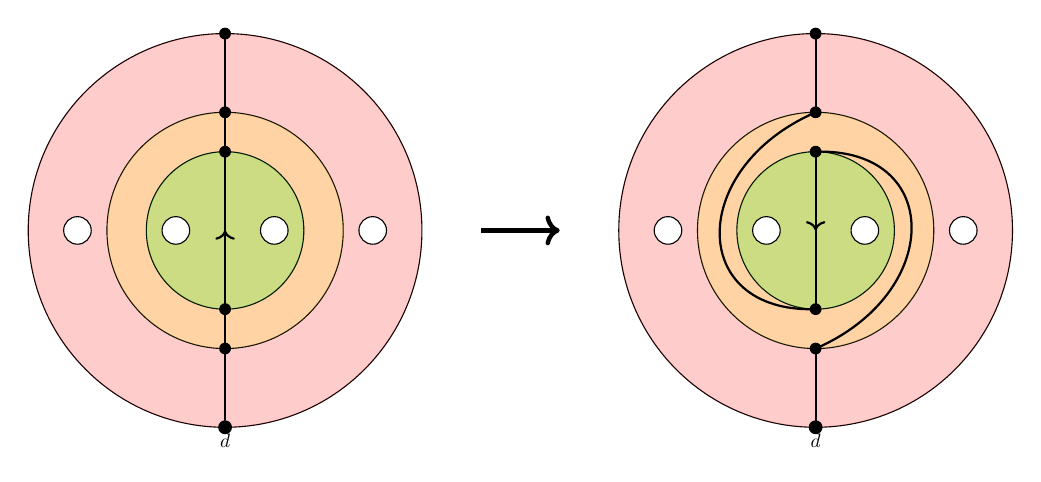
\begin{tikzpicture}[scale=2.5]
                %Left: original punctured disk
                % Large most circle
                \draw (0,0) circle (1); % big circle
                \fill[red,opacity=0.2] (0,0) circle (1);

                %middle circle
                \draw (0,0) circle (0.6);
                \fill[yellow, opacity=0.2] (0,0) circle (0.6);

                %small circle
                \draw (0,0) circle (0.4);
                \fill[green, opacity=0.2] (0,0) circle (0.4);

                %indication line
                \draw[thick] (0,0.4) -- (0,1);
                \draw[thick] (0,-1) -- (0,-0.4);
                \draw[thick, ->-=0.5] (0,-0.4) -- (0,0.4);

                %dots along indication arrow
                \foreach \y in {-0.6,-0.4,0.4,0.6,1}
                    \fill[black] (0,\y) circle (0.03);
                
                % Basepoint
                \fill (0,-1) circle (1pt) node[below, scale=0.7] {$d$};
                
                % Punctures
                \foreach \x in {-0.75, -0.25, 0.25, 0.75}
                    \fill[white] (\x,0) circle (0.07);
                \foreach \x in {-0.75, -0.25, 0.25, 0.75}
                    \draw (\x,0) circle (0.07);


                %mapping arrows
                \draw[->, ultra thick] (1.3,0) -- (1.7,0);


                %Right: twisted punctured disk (everything except the arrow, shifted by x+3
                % Large most circle
                \draw (3,0) circle (1); % big circle
                \fill[red,opacity=0.2] (3,0) circle (1);

                %middle circle
                \draw (3,0) circle (0.6);
                \fill[yellow, opacity=0.2] (3,0) circle (0.6);

                %small circle
                \draw (3,0) circle (0.4);
                \fill[green, opacity=0.2] (3,0) circle (0.4);

                %indication arrow
                \draw[thick,->-=0.5] (3,0.4) -- (3,-0.4);
                \draw[thick] (3,-1) -- (3,-0.6);
                \draw[thick] (3,0.6) -- (3,1);
                \draw[thick] 
                    (3,-0.4) .. controls (2.35,-0.42) and (2.35,0.318) .. (3,0.6);
                \draw[thick] 
                    (3,0.4) .. controls (3.65,0.42) and (3.65,-0.318) .. (3,-0.6);

                %dots along indication arrow
                \foreach \y in {-0.6,-0.4,0.4,0.6,1}
                   \fill[black] (3,\y) circle (0.03);
                
                % Basepoint
                \fill (3,-1) circle (1pt) node[below, scale=0.7] {$d$};
                
                % Punctures
                \foreach \x in {2.25, 2.75, 3.25, 3.75}
                    \fill[white] (\x,0) circle (0.07);
                \foreach \x in {2.25, 2.75, 3.25, 3.75}
                    \draw (\x,0) circle (0.07);
            \end{tikzpicture}
            
            \textbf{Figure:} For $n=4$, Half Twist $\tau_2$ Swapping Punctures $2$ and $3$
        \end{center}

        \textbf{Property:} \emph{Half Twists} $\tau_1,...,\tau_{n-1}$ generates $\mathfrak{M}(D_n)$ and satisfies \emph{Braid Relations}; in fact, $B_n \cong \mathfrak{M}(D_n)$, by $\sigma_i \mapsto \tau_i$.
    }

    \block{Fundamental Group of $D_n$ \& Braid Automorphism}{
        For $n$-punctured disk $D_n$, fix $d \in \partial D$, the fundamental group $\pi_1(D_n, d)$ is generated by the $n$ loops, each surrounding a puncture, which $\pi_1(D_n,d) = F_n(x_1,...,x_n)$, the \emph{Degree-$n$ Free Group}.

        \begin{center}
            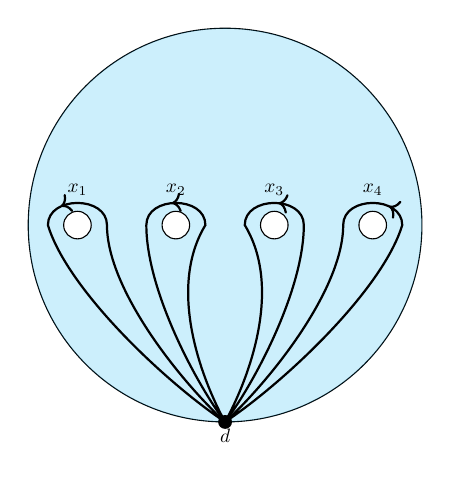
\begin{tikzpicture}[scale=2.5]
                \draw (0,0) circle (1); % big circle
            
                % Shading inside the disk
                \fill[cyan,opacity=0.2] (0,0) circle (1);
                
                % Basepoint
                \fill (0,-1) circle (1pt) node[below, scale=0.7] {$d$};
                
                % Punctures
                \foreach \x in {-0.75, -0.25, 0.25, 0.75}
                    \fill[white] (\x,0) circle (0.07);
                \foreach \x in {-0.75, -0.25, 0.25, 0.75}
                    \draw (\x,0) circle (0.07);
                
                % Loops from basepoint to punctures
                \draw[->-=0.5, thick] (0,-1) .. controls (-0.22,-0.8) and (-0.6,-0.33) .. (-0.6,0) .. node[above, scale=0.7]{$x_1$} controls (-0.6,0.15) and (-0.9,0.15) .. (-0.9,0) .. controls (-0.8,-0.33) and (-0.3,-0.8) .. (0,-1); %left most
                \draw[thick, ->-=0.5] (0,-1) .. controls (0.3,-0.8) and (0.8,-0.33) .. (0.9,0) .. node[above, scale=0.7]{$x_4$} controls (0.9, 0.15) and (0.6, 0.15) .. (0.6,0) .. controls (0.6, -0.33) and (0.22,-0.8) .. (0,-1); %right most (mirror of left most)
                \draw[->-=0.5, thick] (0,-1) .. controls (-0.11,-0.8) and (-0.3,-0.33) .. (-0.1,0) .. node[above, scale=0.7]{$x_2$} controls (-0.1,0.15) and (-0.4,0.15) .. (-0.4,0) .. controls (-0.4,-0.33) and (-0.15,-0.8) .. (0,-1); %middle left
                \draw[thick, ->-=0.5] (0,-1) .. controls (0.15,-0.8) and (0.4,-0.33) .. (0.4,0) .. node[above, scale=0.7]{$x_3$} controls (0.4,0.15) and (0.1,0.15) .. (0.1,0) .. controls (0.3,-0.33) and (0.11,-0.8) .. (0,-1); %middle right (mirror of middle left)
            \end{tikzpicture}

            \textbf{Figure:} Fundamental Group of $D_4$
        \end{center}

        Then, each homeomorphism in $\mathfrak{M}(D_n)$ generates a group automorphism on $\pi_1(D_n,d)$, called \emph{Braid Automorphism}.

        %insert changes of loops. Consider this: https://ncatlab.org/nlab/show/braid+group
        %\textbf{Insert Loop diagrams after half twist}
        \textbf{Ex:} Half Twist's action on $\pi_1(D_n,d)$:
        \[(\tau_i)_*\in \mathrm{Aut}(\pi_1(D_n,d)),\quad (\tau_i)_*(x_j) = \begin{cases}
            x_{i+1} & j=i\\
            x_{i+1}x_ix_{i+1}^{-1} & j=i+1\\
            x_i & \textmd{Otherwise}
        \end{cases}\]

        %Note: Depends on the chosen basepoint, the braid automorphism has a chance of being the inverse instead of the one noted above. Need to work out the details based on personal preference
        \begin{center}
            %try input a braid 
            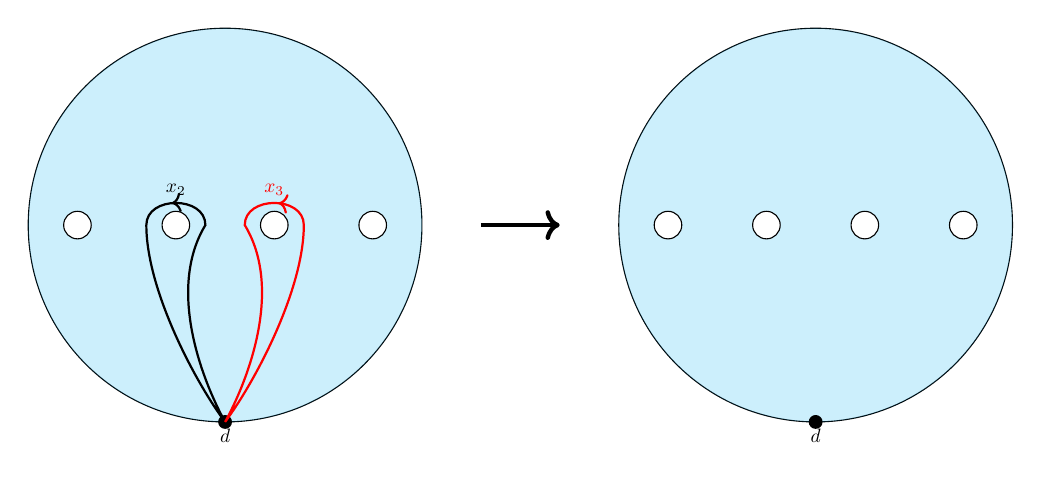
\begin{tikzpicture}[scale=2.5]
                %left circle, before twisted
                \draw (0,0) circle (1); % big circle
            
                % Shading inside the disk
                \fill[cyan,opacity=0.2] (0,0) circle (1);
                
                % Basepoint
                \fill (0,-1) circle (1pt) node[below, scale=0.7] {$d$};
                
                % Punctures
                \foreach \x in {-0.75, -0.25, 0.25, 0.75}
                    \fill[white] (\x,0) circle (0.07);
                \foreach \x in {-0.75, -0.25, 0.25, 0.75}
                    \draw (\x,0) circle (0.07);
                
                % Loops from basepoint to punctures
                \draw[->-=0.5, thick] (0,-1) .. controls (-0.11,-0.8) and (-0.3,-0.33) .. (-0.1,0) .. node[above, scale=0.7]{$x_2$} controls (-0.1,0.15) and (-0.4,0.15) .. (-0.4,0) .. controls (-0.4,-0.33) and (-0.15,-0.8) .. (0,-1); %middle left
                \draw[red, thick, ->-=0.5] (0,-1) .. controls (0.15,-0.8) and (0.4,-0.33) .. (0.4,0) .. node[above, scale=0.7]{$x_3$} controls (0.4,0.15) and (0.1,0.15) .. (0.1,0) .. controls (0.3,-0.33) and (0.11,-0.8) .. (0,-1); %middle right (mirror of middle left)


                %arrow
                \draw[ultra thick, ->] (1.3,0) -- (1.7,0);

                
                %right side, twisted 
                \draw (3,0) circle (1); % big circle
            
                % Shading inside the disk
                \fill[cyan,opacity=0.2] (3,0) circle (1);
                
                % Basepoint
                \fill (3,-1) circle (1pt) node[below, scale=0.7] {$d$};
                
                % Punctures
                \foreach \x in {2.25, 2.75, 3.25, 3.75}
                    \fill[white] (\x,0) circle (0.07);
                \foreach \x in {2.25, 2.75, 3.25, 3.75}
                    \draw (\x,0) circle (0.07);
                
                % Loops from basepoint to punctures
                %\draw[thick, ->-=0.5] (0,-1) .. controls (0.15,-0.8) and (0.4,-0.33) .. (0.4,0) .. node[above, scale=0.7]{$x_3$} controls (0.4,0.15) and (0.1,0.15) .. (0.1,0) .. controls (0.3,-0.33) and (0.11,-0.8) .. (0,-1); %x_2 sends to x_3
            \end{tikzpicture}

            \textbf{Figure:} $\tau_2$ Action on Loops in $D_4$
        \end{center}
        %The collection of $(\tau_i)_*$ again satisfies the Braid Relations, which generates a group homomorphism $B_n \rightarrow \mathrm{Aut}(\pi_1(D_n, d))$ by $\sigma_i \mapsto (\tau_i)_*$; this homomorphism is injective, so the braid group of $n$ strands $B_n$ is a subgroup of $\mathrm{Aut}(\pi_1(D_n, d))$.
    }
    
    \column{0.36}  
    \block{Reduced Burau Representation}{
        $\psi_n^r:B_n \rightarrow \mathrm{GL}_{n-1}(\mathbb{Z}[t^\pm])$ satisfies:
        $$\sigma_1\mapsto \left(\begin{array}{cc|c}
            -t & 0 & 0 \\
             1 & 1 & 0 \\
             \hline 
             0 & 0 & I_{n-3}
        \end{array}\right),\ \sigma_{n-1}\mapsto \left(\begin{array}{c|cc}
            I_{n-3} & 0 & 0\\
            \hline 
            0 & 1 & t\\
            0 & 0 & -t
        \end{array}\right),\ \sigma_i\mapsto \left(\begin{array}{c|ccc|c}
            I_{i-2} & 0 & 0 & 0 & 0\\
            \hline
            0 & 1 & t & 0 & 0\\
            0 & 0 & -t & 0 & 0\\
            0 & 0 & 1 & 1 & 0\\
            \hline
            0 & 0 & 0 & 0 & I_{n-i-2}
        \end{array}\right)$$
    }

    \block{Ex: Homological Perspective on $D_4$}{
        A $4$-punctured disk $D_4$ can "continuously deform" into $4$ circles joining at one point ($\bigvee_{i=1}^4S^1$), $\implies$ Same Fundamental Group.

        \begin{center}
            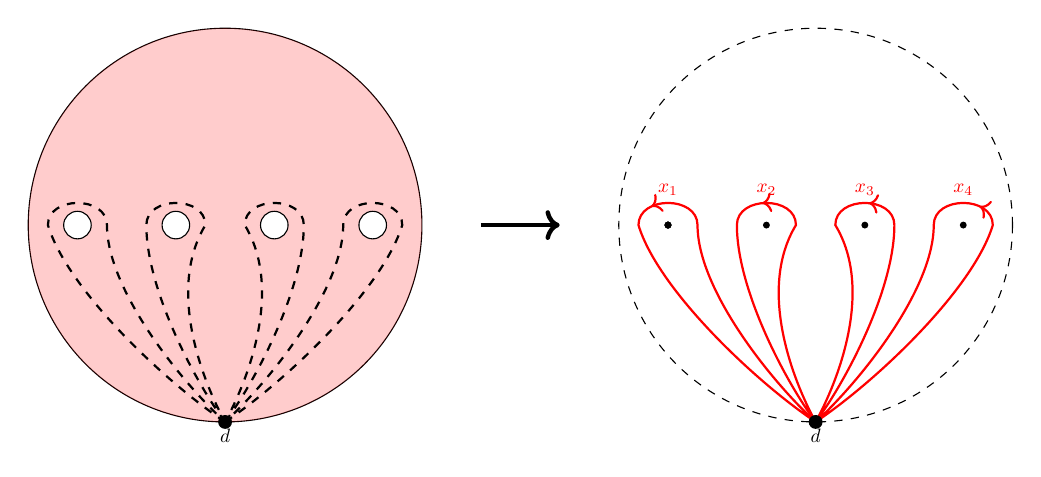
\begin{tikzpicture}[scale=2.5]
            % Left side: punctured disk
            \draw (0,0) circle (1); % big circle
            
            % Shading inside the disk
            \fill[red,opacity=0.2] (0,0) circle (1);
            
            % Basepoint
            \fill (0,-1) circle (1pt) node[below, scale=0.7] {$d$};
            
            % Punctures
            \foreach \x in {-0.75, -0.25, 0.25, 0.75}
                \fill[white] (\x,0) circle (0.07);
            \foreach \x in {-0.75, -0.25, 0.25, 0.75}
                \draw (\x,0) circle (0.07);
            
            % Loops from basepoint to punctures
            \draw[dashed, thick] (0,-1) .. controls (-0.3,-0.8) and (-0.8, -0.33) .. (-0.9, 0) .. controls (-0.9,0.15) and (-0.6, 0.15) .. (-0.6,0) .. controls (-0.6, -0.33) and (-0.22,-0.8) .. (0,-1); %left most
            \draw[dashed, thick] (0,-1) .. controls (0.3,-0.8) and (0.8,-0.33) .. (0.9,0) .. controls (0.9, 0.15) and (0.6, 0.15) .. (0.6,0) .. controls (0.6, -0.33) and (0.22,-0.8) .. (0,-1); %right most (mirror of left most)
            \draw[dashed, thick] (0,-1) .. controls (-0.15,-0.8) and (-0.4,-0.33) .. (-0.4,0) .. controls (-0.4,0.15) and (-0.1,0.15) .. (-0.1,0) .. controls (-0.3,-0.33) and (-0.11,-0.8) .. (0,-1); %middle left
            \draw[dashed, thick] (0,-1) .. controls (0.15,-0.8) and (0.4,-0.33) .. (0.4,0) .. controls (0.4,0.15) and (0.1,0.15) .. (0.1,0) .. controls (0.3,-0.33) and (0.11,-0.8) .. (0,-1); %middle right (mirror of middle left)
            

            % Arrow between pictures
            \draw[->,ultra thick] (1.3,0) -- (1.7,0);
            

            % Right side: wedge of circles
            \draw[dashed] (3,0) circle (1);
            
            % Wedge loops
            \draw[red, ->-=0.5, thick] (3,-1) .. controls (2.78,-0.8) and (2.4,-0.33) .. (2.4,0) .. node[above, scale=0.7]{$x_1$} controls (2.4,0.15) and (2.1,0.15) .. (2.1,0) .. controls (2.2,-0.33) and (2.7,-0.8) .. (3,-1); %left most
            %\draw[red, ->-=-0.5, thick] (3,-1) .. controls (2.85,-0.8) and (2.6,-0.33) .. (2.6,0) .. node[above, scale=0.7] {$x_2$} controls (2.6,0.15) and (2.9,0.15) .. (2.9,0) .. controls (2.7,-0.33) and (2.89,-0.8) .. (3,-1); %middle left
            \draw[red, ->-=0.5, thick] (3,-1) .. controls (2.89,-0.8) and (2.7,-0.33) .. (2.9,0) .. node[above, scale=0.7]{$x_2$} controls (2.9,0.15) and (2.6,0.15) .. (2.6,0) .. controls (2.6,-0.33) and (2.85,-0.8) .. (3,-1); %middle left
            \draw[red, ->-=0.5, thick] (3,-1) .. controls (3.15,-0.8) and (3.4,-0.33) .. (3.4,0) .. node[above, scale=0.7] {$x_3$} controls (3.4,0.15) and (3.1,0.15) .. (3.1,0) .. controls (3.3,-0.33) and (3.11,-0.8) .. (3,-1); %middle right (mirror of middle left)
            \draw[red, ->-=0.5, thick] (3,-1) .. controls (3.3,-0.8) and (3.8,-0.33) .. (3.9,0) .. node[above, scale=0.7] {$x_4$} controls (3.9, 0.15) and (3.6, 0.15) .. (3.6,0) .. controls (3.6, -0.33) and (3.22,-0.8) .. (3,-1); %right most (mirror of left most)

            % Basepoint of second graph
            \fill (3,-1) circle (1pt) node[below, scale=0.7] {$d$};
            
            % Small dots at loop tops
            \foreach \x in {2.25, 2.75, 3.25, 3.75}
            \fill[black] (2.25,0) circle (0.5pt);
            \fill[black] (2.75,0) circle (0.5pt);
            \fill[black] (3.25,0) circle (0.5pt);
            \fill[black] (3.75,0) circle (0.5pt);
        \end{tikzpicture}
        
            \textbf{Figure:} Deformation Retraction of $D_4$ to $\bigvee_{i=1}^4 S^1$
        \end{center} %change the direction of the arrow

        Let $S^{(4)} := \bigvee_{i=1}^4 S^1$, consider the space $\tilde{S}^{(4)}$ below, a \emph{Covering Space} of $S^{(4)}$:

        \begin{center}
            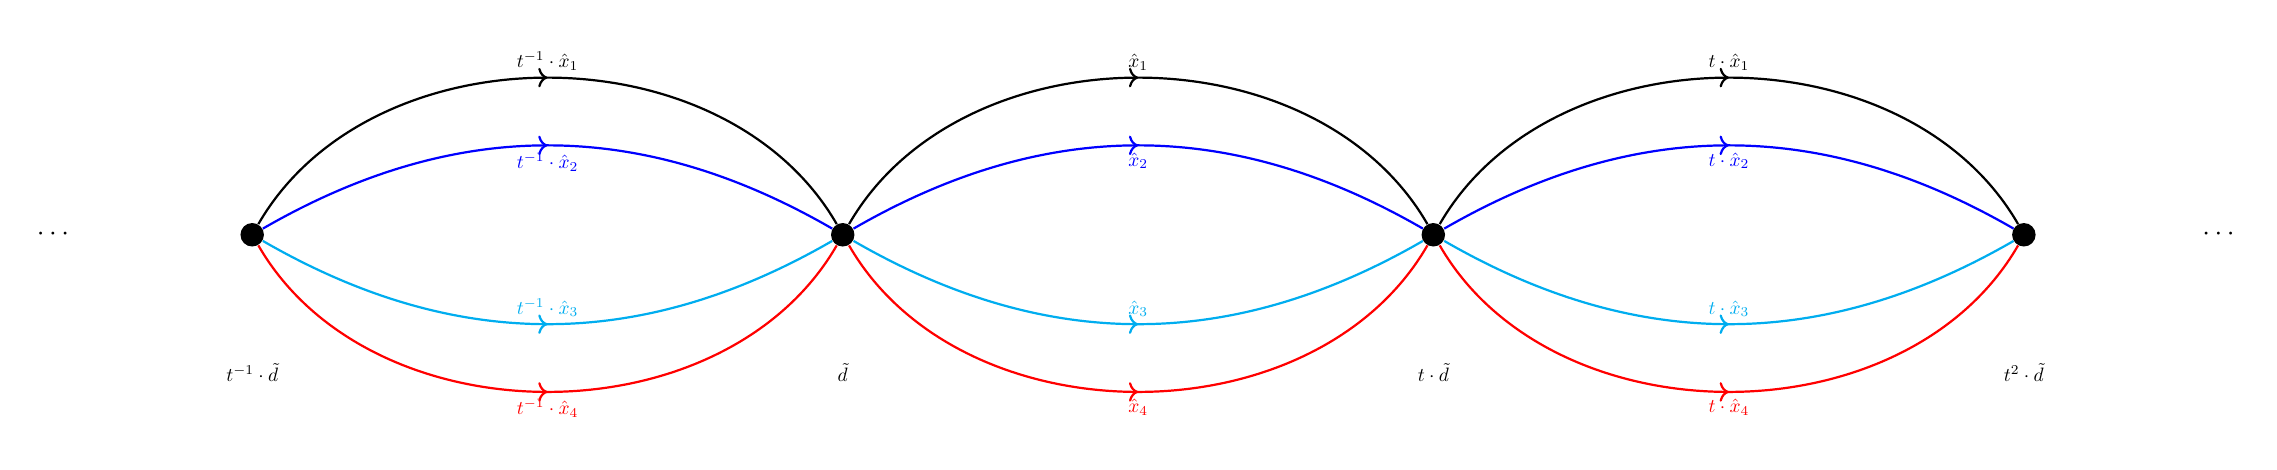
\begin{tikzpicture}[scale=2.5]
            % coordinates for the nodes
            \node (A) at (0,0) [circle,fill,inner sep=3pt]{};
            \node (B) at (3,0) [circle,fill,inner sep=3pt]{};
            \node (C) at (6,0) [circle,fill,inner sep=3pt]{};
            \node (D) at (9,0) [circle,fill,inner sep=3pt]{};
            
            % left loops (t^{-1})
            \draw[->-=0.5, thick] (A) to[out=60,in=120] node[above, scale=0.7]{$t^{-1}\cdot \hat{x}_{1}$} (B);
            \draw[->-=0.5, blue, thick] (A) to[out=30,in=150] node[below, scale=0.7]{$t^{-1}\cdot \hat{x}_{2}$} (B);
            \draw[->-=0.5, cyan, thick] (A) to[out=-30,in=-150] node[above, scale=0.7]{$t^{-1}\cdot \hat{x}_{3}$} (B);
            \draw[->-=0.5, red, thick] (A) to[out=-60,in=-120] node[below, scale=0.7]{$t^{-1}\cdot \hat{x}_{4}$} (B);
            
            % middle loops (1)
            \draw[->-=0.5, thick] (B) to[out=60,in=120] node[above, scale=0.7]{$\hat{x}_{1}$} (C);
            \draw[->-=0.5, blue, thick] (B) to[out=30,in=150] node[below, scale=0.7]{$\hat{x}_{2}$} (C);
            \draw[->-=0.5, cyan, thick] (B) to[out=-30,in=-150] node[above, scale=0.7]{$\hat{x}_{3}$} (C);
            \draw[->-=0.5, red, thick] (B) to[out=-60,in=-120] node[below, scale=0.7]{$\hat{x}_{4}$} (C);
            
            % right loops (t)
            \draw[->-=0.5, thick] (C) to[out=60,in=120] node[above, scale=0.7]{$t\cdot \hat{x}_{1}$} (D);
            \draw[->-=0.5, blue, thick] (C) to[out=30,in=150] node[below, scale=0.7]{$t\cdot\hat{x}_{2}$} (D);
            \draw[->-=0.5, cyan, thick] (C) to[out=-30,in=-150] node[above, scale=0.7]{$t\cdot\hat{x}_{3}$} (D);
            \draw[->-=0.5, red, thick] (C) to[out=-60,in=-120] node[below, scale=0.7]{$t\cdot\hat{x}_{4}$} (D);
            
            % labels under bottom arcs
            \node[scale=0.7] at (0,-0.7) {$t^{-1}\cdot\tilde d$};
            \node[scale=0.7] at (3,-0.7) {$\tilde d$};
            \node[scale=0.7] at (6,-0.7) {$t\cdot\tilde d$};
            \node[scale=0.7] at (9,-0.7) {$t^2\cdot\tilde d$};
            
            % dots on ends
            \node at (-1,0) {$\cdots$};
            \node at (10,0) {$\cdots$};
            \end{tikzpicture}

            \textbf{Figure:} Infinite Cyclic Cover $\tilde{S}^{(4)}$
        \end{center}
        Here, $t$ is a right shift of $\tilde{S}^{(n)}$ by degree $1$:
        \begin{itemize}
            \item $t^k\cdot \tilde{d} = $ degree $k$ right shift of $\tilde{d}$
            \item $t^k\cdot \hat{x}_i = $ degree $k$ right shift of $\hat{x}_i$
        \end{itemize}
        There is a continuous covering map $p:\tilde{S}^{(4)}\rightarrow S^{(4)}$, each $p(t^k \cdot \hat{x}_{i}) = x_i$, and $p(t^k \cdot \tilde{d}) = d$.
        
        Define the "Base Loops" $\ell_i := \hat{x}_{i+1}\cdot \hat{x}_i^{-1}$ (counterclockwise) for $1\leq i\leq 3$:
        \begin{itemize}
            \item $-\ell_i = $ clockwise version of $\ell_i$
            \item $t^k \cdot \ell_i = $ degree $k$ right shift of $\ell_i$
        \end{itemize}
        Then, all "Integer Laurent Polynomial" combination of $\ell_i$ forms $H_1(\tilde{S}^{(4)})$ as a free $\mathbb{Z}[t^\pm]$-module with basis $\ell_1,\ell_2,\ell_3$.
    }

    \column{0.32}

    \block{Braid Group's Action on Covering Space}{
        \textbf{Recall:} braid automorphism $(\tau_2)_*$ of $\pi_1(D_4,d)$ satisfies $(\tau_2)_*(x_2) = x_3$, and $(\tau_2)_*(x_3) = x_3\cdot x_2\cdot x_3^{-1}$. Which, it uniquely lifts to an transformation on the $\ell_i$ via $p$: 
        
        \textbf{EX:} $\ell_2 = \hat{x}_{3}\cdot \hat{x}_{2}^{-1} \mapsto \hat{x}_{2} \cdot \left((t\cdot \hat{x}_{2})\cdot (t\cdot \hat{x}_{3}^{-1})\cdot \hat{x}_{2}^{-1}\right) = -t \cdot \ell_2$.
        
        \begin{center}
            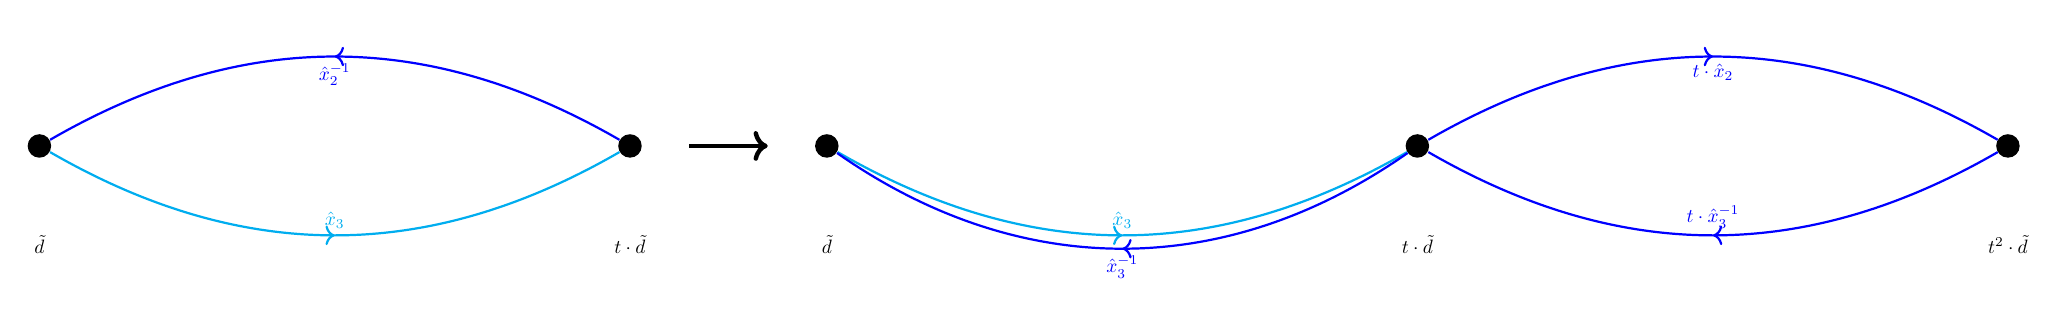
\begin{tikzpicture}[scale=2.5]
                %First graph about \ell_2, define nodes first
                \node (A) at (0,0) [circle,fill,inner sep=3pt]{};
                \node (B) at (3,0) [circle,fill,inner sep=3pt]{};

                %Draw the loop's associated orientation
                \draw[->-=0.5, blue, thick] (B) to[out=150,in=30] node[below, scale=0.7]{$\hat{x}_{2}^{-1}$} (A);
                \draw[->-=0.5, cyan, thick] (A) to[out=-30,in=-150] node[above, scale=0.7]{$\hat{x}_{3}$} (B);

                %label the dots in the first graph
                \node[scale=0.7] at (0,-0.5) {$\tilde d$};
                \node[scale=0.7] at (3,-0.5) {$t\cdot\tilde d$};


                %intermediate arrow
                \draw[->,ultra thick] (3.3,0) -- (3.7,0);


                %next graph aboug where \ell_2 gets mapped to, define nodes first again
                \node (C) at (4,0) [circle,fill,inner sep=3pt]{};
                \node (D) at (7,0) [circle,fill,inner sep=3pt]{};
                \node (E) at (10,0) [circle,fill,inner sep=3pt]{};

                %first path where x_{3,1} gets mapped to
                \draw[->-=0.5, cyan, thick] (C) to[out=-30,in=-150] node[above,scale=0.7]{$\hat{x}_{3}$} (D);

                %second path where x_{2,1}^{-1} gets mapped to
                \draw[->-=0.5, blue, thick] (D) to[out=30,in=150] node[below,scale=0.7]{$t\cdot \hat{x}_{2}$} (E);
                \draw[->-=0.5, blue, thick] (E) to[out=-150,in=-30] node[above,scale=0.7]{$t\cdot \hat{x}_{3}^{-1}$} (D);
                \draw[->-=0.5, blue, thick] (D) to[out=-145,in=-35] node[below,scale=0.7]{$\hat{x}_{3}^{-1}$} (C);

                %label the dots in the second graph
                \node[scale=0.7] at (4,-0.5) {$\tilde d$};
                \node[scale=0.7] at (7,-0.5) {$t\cdot\tilde d$};
                \node[scale=0.7] at (10,-0.5) {$t^2\cdot\tilde d$};
            \end{tikzpicture}

            \textbf{Figure:} $\ell_2$ (Counterclockwise) Maps to $-t\cdot \ell_2$ (Right Shift by degree 1, Clockwise)
        \end{center}
        Doing this for each $\ell_i$, put into matrix form with basis $\{\ell_i\}$, we recover the Representation.
    }

    \block{Gassner Representation}{
        Instead of on braid groups $B_n$, this one is representing \emph{Pure Braid Group} $P_n$: Given the map $B_n \rightarrow S_n$ ($n^\textmd{th}$ Symmetry Group) by $\sigma_i\mapsto (i, i+1)$, $P_n$ is the kernel of this morphism (Geometrically, it's the braids with the strand going from the $i^\textmd{th}$ starting point to the $i^\textmd{th}$ ending point, which forms identity as a permutation of the $n$ endpoints).

        If consider the covering map corresponding to the kernel of $\pi_1(S^{(n)},d) \rightarrow \mathbb{Z}^n$ by $x_i \mapsto e_i$ (the $i^\textmd{th}$ basis of $\mathbb{Z}^n$), it forms a representation $P_n \rightarrow \mathrm{GL}_n(\mathbf{Z}[t_1^\pm,...,t_n^\pm])$.
    }

    \block{Conclusion \& Future Directions}{}
    \block{Acknowledgement \& Sources}{
        We're genuinely thankful for the parent donors, Professor Cachadina and Professor Casteels who made this program possible. 
        We also want to thank our mentor Choomno Moos for their great guidance.
        \vspace{-0.3cm}
        \begin{itemize}
            \item Braid Groups (Christian Kassel, Vladimir Turaev)
            \item Algebraic Topology (Hatcher)
            \item Braids, Links, Mapping Class Groups (Joan Birman)
            %\item Introduction to Topological Manifold (John Lee)
            %\item An Introduction to Knot Theory (W.B. Raymond Lickorish)
            %\item Category Theory in Context (Emily Riehl)
            %\item Algebra Chapter 0 (Paolo Aluffi)
        \end{itemize}
    }
\end{columns}
\end{document}